\chapter{Recovery}

事务主要包含两个大的功能：并发与恢复，上一章介绍了事务的并发控制，本章讨论事务的恢复。

\section{故障模型}

单机故障模型假设数据库系统运行在一个单机上，故障发生，系统崩溃，当系统重启，系统回滚恢复到崩溃前的状态，所有未完成事务被放弃。而在云计算中，要求提供7*24小时的服务，这就要求数据库系统必须要提供高可用性，即系统崩溃后，能够快速恢复到正常状态。

单机故障恢复主要依赖于日志WAL，在系统重启后，先分析日志，找到最近的checkpoint，然后从checkpoint后的日志开始回放，恢复状态。云计算的系统主要依赖于冗余提供高可用性，某个节点崩溃，其它可用节点能够快速接管，提供服务。云计算中的节点仍然高度依赖日志回放，副本节点通过全局日志回放接管服务。

单机故障模型和云计算故障模型的区别是明显的，前者依赖于持久化存储设备上的日志，后者还依赖于心跳+Paxos协议等来实现全局状态的一致。本章的内容主要讨论单机故障模型的恢复，云计算故障模型的恢复会在后续章节介绍。

\begin{exercise}
    单机故障模型下，认为日志总是是可靠的。实际系统中，日志也不一定总是可靠的，如何保证日志的可靠性？
\end{exercise}

\subsection{扩展行模型}

在单机故障中，系统恢复的是已提交的事务，未提交的事务被回滚。回滚要撤销该事务的所有修改，将数据库恢复到事务开始前的状态，它是一个逆操作。我们仍然从简单的模型开始讨论，先讨论行模型的回滚，然后再讨论对象模型的回滚。

行模型有两个操作，读和写，其中只有写操作会对行做修改，因此只有写操作需要实现逆操作。行模型是一个抽象模型，写的逆操作是恢复之前的行。考虑下面的一个调度：
$$
s = r_1(x)w_1(x)r_2(x)a_1w_2(x)c_2
$$
这个调度中，$t_1$事务回滚，要撤销之前的修改，将$x$恢复到$w_1(x)$之前的状态，$a_1$会执行逆操作$w_1^{-1}(x)$，其实际执行的调度是：
$$
s' = r_1(x)w_1(x)r_2(x)w_1^{-1}c_1(x)w_2(x)c_2
$$
在本章的讨论中，形式化的调度在上一章并发控制的基础上，增加了提交和取消两个动作，取消或者回滚可以扩展为写操作的逆操作，然后归结于正常提交。

\subsection{行模型的可恢复性}

在调度中引入提交和取消动作，扩展了行模型。要判读一个扩展行模型的并发是否正确，仍然要看它是否冲突等价于一个串行化执行的调度。

\begin{example}\label{ex:8-recover}
考虑如下调度：
$$
s = r_1(x)w_1(x)r_2(x)a_1c_2
$$
这个例子中，$t_2$脏读了$x$。$s$的冲突集是$conf(s)=\{ (w_1(x),r_2(x))\}$，它的扩展调度是：
$$
s' = r_1(x)w_1(x)r_2(x)w_1^{-1}(x)c_1c_2
$$
无需考虑逆操作的冲突，$s'$的冲突集是$conf(s')=\{ (w_1(x),r_2(x))\}$，与$conf(s)$相同。但$t_1$的写操作$w_1(x)$已经被取消，这个调度有问题。
\end{example}

在处理扩展行模型时，取消操作$a$可以将整个事务的所有操作全部删除，删除后的等价冲突集不变。

\begin{example}\label{ex:8-recover2}
    考虑如下调度：
$$
s=r_1(x)w_1(x)r_2(x)w_2(x)a_2a_1
$$
它等价于如下的调度：
\begin{align*}
s' &= r_1(x)w_1(x)r_2(x)w_2(x)w_2^{-1}(x)c_2a_1 \\
   &= r_1(x)w_1(x)r_2(x)c_2a_1 \\
   &= r_1(x)w_1(x)c_2a_1 \\
   &= r_1(x)w_1(x)c_2w_1^{-1}(x)c_1 \\
   &= r_1(x)c_2c_1 \\
   &= c_2c_1
\end{align*}
\end{example}

仔细观察两个例子，\examplename\ref{ex:8-recover2}能正常恢复，而\examplename\ref{ex:8-recover}是有问题的。本章引入扩展行模型的的目的是为了讨论事务的恢复，\examplename\ref{ex:8-recover}是不可恢复的。这里不形式化定义可恢复性，可以参考\cite{Weikum2001Transactional}。

一个基本常识：如果扩展行模型的所有事务正常提交，或者说可串行化，那么以逆序方式取消事务，得到的调度是可恢复的。

\examplename\ref{ex:8-recover}的脏读例子，为了使得调度正确，需要使得$t_2$被回滚，这称为级联回滚。一般来说，级联回滚会使得系统的恢复时间增加，因此在设计数据库系统时，要尽量避免级联回滚。

\subsection{对象模型}

在上一章讨论事务并发时，我们引入了对象模型：我们假设，高层事务接口被分解为几个层次，最后一层是行模型。对象模型调度的正确性依赖于底层行模型的正确性，对象模型的可恢复性类似，我们寄望于底层行模型上能够实现可恢复性，那么对象模型的调度也是可恢复的。

在高层实现逆操作，开销非常大，设计难度很高，对象模型可恢复性由底层行模型实现是非常美好的。但是，这一原则并不总是有效，因为系统内总有些高层事务接口无法映射为行模型，例如对数据库文件页面的操作，操作的对象是页面而非抽象的行，要处理页面分裂合并等问题。

\section{wal}

上一节我们简单讨论了事务恢复在行模型上的可恢复性，技术上，在单机模型上实现逆操作需要日志的支持。因为取消动作并不只在并发才有，在系统恢复也会用到。基于日志的恢复方案主要源自ARIES\cite{mohan1992aries}，ARIES规范了恢复流程，解耦了并发与恢复，讨论了checkpoint的实现等。

数据库为了恢复，任何对数据库内部对象的修改，都要先记录日志，这称为write ahead logging（WAL）。WAL的实现一般要求文件系统支持journaling，并且由于日志是追加写入，日志条目的增加虽然变长，但是原子的。底层文件系统journalling机制的要求其实不低，从文件系统的发展来看，这个机制的完整实现都是很后来的事情了。

随着SSD器件的普及，wal的实现变得要简单一些\cite{GitHubgo38:online}，因为SSD内部有一套虚拟块号映射机制，追加写入要先分配一块新的地址，擦除原物理地址。

\subsection{物理日志与逻辑日志}

WAL记录的信息用于恢复系统，数据库系统是分层次的，底层是存储系统，上层是执行引擎、事务引擎等。日志需要记录哪些信息？从目前众多数据库的选择来看，不约而同选择底层存储系统的变化作为日志信息。其中的道理可以类比前述的对象模型，高层对象的操作最终会分解为底层存储系统上的操作。

一般而言，物理日志记录的是底层存储系统的变化，逻辑日志记录的是高层事务接口的变化。数据库日志一般以物理日志为主，但并不排除跨层记录的情形，例如2PC协议，prepare阶段需要记录状态。

\begin{exercise}
    在分布式系统中，存储系统分为share nothing或者share everything两种设计。为了提供7*24不间断服务，一般会采用Paxos/Raft协议提供冗余，这些协议是否要记录日志？
\end{exercise}

在ARIES的设计中，基本上是以buffer管理为界线，如\figurename\ref{fig:1-arch}，其上为高层，其下是存储系统。可以说，ARIES是面向存储系统的日志机制。

这里有必要再回顾一下，前述的事务并发控制基于行模型，行模型是一个高层的逻辑模型。而日志系统是针对底层存储系统设计，两者之间有明显的设计差异。在后面的内容中，要注意观察高层的恢复需求是如何体现在底层日志系统的设计上的。

\subsection{日志的结构}

日志是有结构的，正如第\ref{chap:layout}章的记录。按照ARIES的方案\cite{mohan1992aries}，一个日志条目包含如下字段，这些字段设计的必要性在后介绍。

\begin{itemize}
    \item LSN：日志条目编号，全局唯一，递增。有些系统中的LSN是日志文件中的偏移量，在日志条目中并没有这个字段。oracle数据库中，SCN是一个逻辑时戳。
    \item checksum：校验和，用于检查日志是否损坏。
    \item length：日志条目长度。
    \item type：日志类型，update、compensation、checkpoint、prepare等。
    \item tid+prevLSN：事务号以及该事务的前一个日志条目编号，用于构建事务的日志链。
    \item pageid：页面编号。
    \item undoNxtLSN：补偿日志的指针。
    \item data：日志载荷。
\end{itemize}

\begin{exercise}
    Oracle的SCN为什么设计为一个逻辑时戳？
\end{exercise}

从设计的弹性来看，一般用type来标记特定的函数对象，data标记函数对象的调用参数，如\figurename\ref{fig:8-wal}所示，其中payload部分的设计模仿第\ref{chap:layout}章的记录。

\begin{figure}[H]
    \centering
    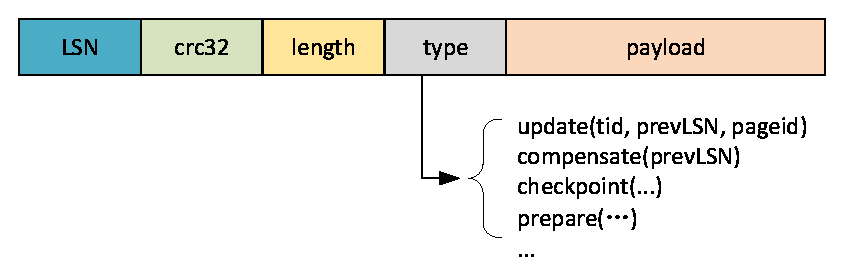
\includegraphics[width=0.8\linewidth]{handout/img/8-wal.eps}
    \caption{WAL日志格式}\label{fig:8-wal}
\end{figure}

日志文件用追加方式写入，多数文件系统会提供原子追加操作。日志条目之间，不用添加特殊分隔符，因为日志条目的扫描从checkpoint开始向后扫，每个条目包含长度信息。如果出现校验损坏，其后的日志条目也是不可信的，要放弃。

\begin{exercise}
    如果扫描日志条目，遇到校验损坏的条目，为什么要放弃后续日志的扫描？
\end{exercise}
\begin{exercise}
    模仿第\ref{chap:layout}章的记录，补充\figurename\ref{fig:8-wal}的payload设计。
\end{exercise}

\section{基本功能}

本节开始讨论日志需要支持的功能及其实现方案，数据库日志的功能设计是具有弹性的，并不是固定的。本讲义从最简单的需求开始，逐步丰富日志的功能，堆砌出一个完整的日志框架。

\subsection{update}

考虑在行模型中，写一行数据如何在底层存储系统上实现。如\figurename\ref{fig:8-update}所示，一个在session运行的事务，要将本地缓冲的行写入一页。先在锁表中加锁，然后对页面上闩，在修改页面之前，先记录日志。

\begin{figure}[H]
    \centering
    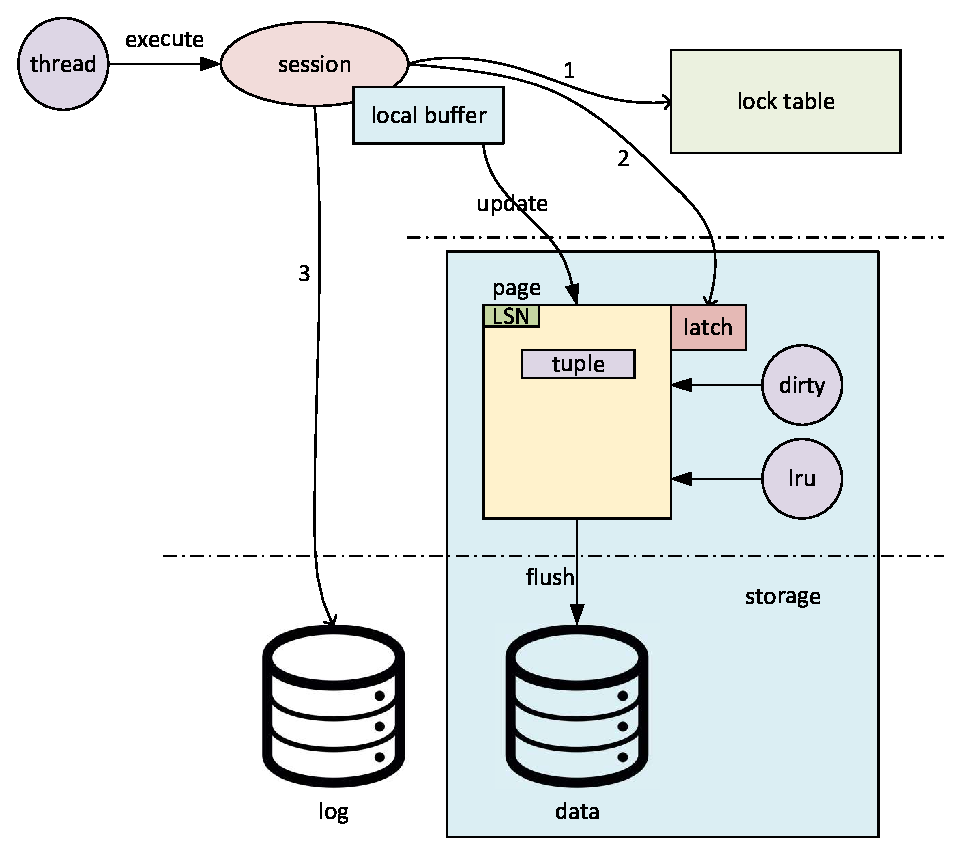
\includegraphics[width=0.8\linewidth]{handout/img/8-update.eps}
    \caption{写一行过程}\label{fig:8-update}
\end{figure}

\begin{exercise}
    \figurename\ref{fig:8-update}所示为锁方案，假设采用第\ref{chap:concurrent}章两种rset维持方案，该如何处理？
\end{exercise}

在锁方案中，对行更新可能会导致死锁，需要一个死锁检测与解锁机制。在mvcc中，由于读锁不会阻塞事务推进，所以不需要死锁检测。\figurename\ref{fig:8-update}对页面加锁也可能会导致闩的死锁，如果采用组提交策略，在提交阶段写入，以first-commit-wins策略可以避免这一问题。——可以看到，mvcc比锁方案先进太多，规避了很多难题。

\figurename\ref{fig:8-update}中，存储引擎包含了缓冲管理、底层存储管理、文件管理等功能，日志是针对这一层设计。页面由缓冲层管理，一般内置脏链、lru链，当缓冲层的页面不敷使用，会下刷dirty页面或者释放干净页面。

另一个值得注意的是，\figurename\ref{fig:8-update}解耦了事务处理与数据刷新。事务对数据的更新只到缓冲层的页面，脏页面的刷新由缓冲管理层负责。

\begin{exercise}
    假设系统不支持脏读，\figurename\ref{fig:8-update}中的latch会导致死锁发生吗？
\end{exercise}

\subsubsection*{undo+redo}

考虑日志的设计，对一个对象的修改，需要记录两个信息：UNDO+REDO。前者用于回滚，后者用于恢复，两类信息是必需的，缺一不可。但在实现中，可以将UNDO和REDO拆开为两条日志，先记录UNDO，然后记录REDO。

\begin{figure}[H]
    \centering
    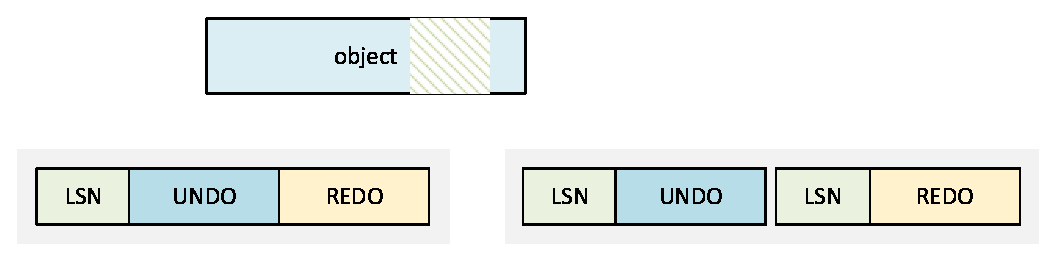
\includegraphics[width=0.8\linewidth]{handout/img/8-modify.eps}
    \caption{undo+redo}\label{fig:8-modify}
\end{figure}

如\figurename\ref{fig:8-modify}所示，对于一个对象的update操作，有两种方案，一种是在一条日志中记录所有UNDO+REDO，另一种是先记录UNDO，然后记录REDO。

\begin{exercise}
    \figurename\ref{fig:8-modify}中，为什么一定要先记录UNDO？可不可以先记录REDO？
\end{exercise}

采用read-only+undo-only的日志方案，需要在type字段补充一些信息。因为在系统恢复阶段，日志会被重放，所以仍然要在undo-only日志中类型中标记update，意思是这个undo日志在更新中不需要执行。

\subsubsection*{页面结构}

日志是针对存储系统设计的，关系型数据的存储都是按页组织的，undo+redo日志中一定会包含pageid，在系统恢复中，这些信息足够了。但是，另一个场景是，一个事务修改了页面，但后来又被取消，页面需要回滚。

要提供页面回滚功能，可以扫描日志，找到对该页面的undo条目，撤销该页面的修改。这个过程太漫长了，为了方便页面的回滚，在页面上设计了一个LSN字段，指向日志条目。

\begin{figure}[H]
    \centering
    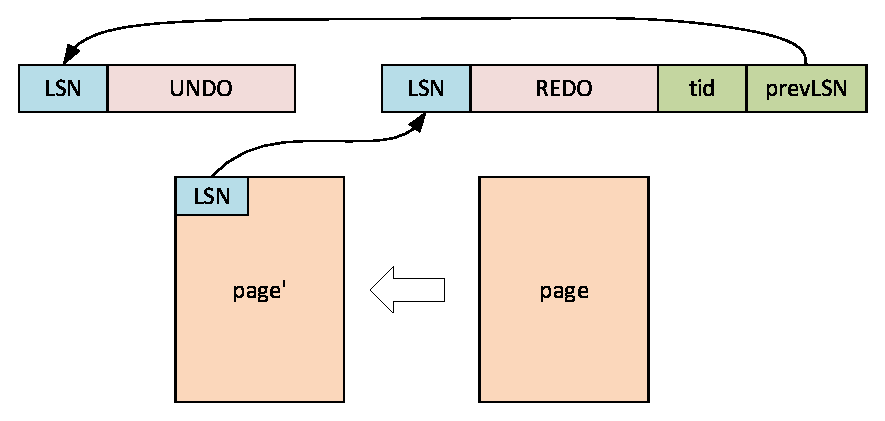
\includegraphics[width=0.7\linewidth]{handout/img/8-prev.eps}
    \caption{事务日志前驱指针}\label{fig:8-prev}
\end{figure}

在\figurename\ref{fig:8-prev}中，为快速定位修改页面的日志条目，在页面结构上增加一个字段LSN。LSN指向修改该页面的REDO日志，REDO日志带上prevLSN指针，指向前一个日志条目，顺着这个逆向链表，可以快速定位该页面的undo日志。

\begin{exercise}
    \figurename\ref{fig:8-prev}中，LSN为什不指向的UNDO日志？
\end{exercise}

从页面LSN字段的设计，可以获得一个技能：要快速回滚某个对象，只需在对象上带上LSN字段即可。\figurename\ref{fig:8-prev}中，prevLSN并不是指向UNDO日志，它实际上维护了一个事务的修改历史链表，这是为了方便事务的管理，日志源一般都是事务。可以看到日志的设计是非常有弹性的，并没有绑死在存储系统上。

\subsection{rollback}

回滚要求撤销事务之前的修改，系统恢复时，需要撤销未完成事务的修改。此外，事务由于并发原因，可能会被取消重启，也需要回滚功能。SQL标准要求实现savepoint，以提供更细粒度的回滚能力，不必撤销整个事务的所有修改，只撤销部分。还有些情况下，允许子事务嵌套，当子事务被取消，也需部分回滚。

回滚的实现，要借助于前述update的undo日志，ARIES中将回滚动作称为补偿日志，compensation log record，CLR。前述的undo日志只是提供了回滚的操作，CLR是执行这个操作的标志。任何对数据库状态的修改，都需记录在案，包括CLR日志。

举例而言，一个系统崩溃，重启后恢复，undo了一些修改，此时再次崩溃，如果不记录CLR日志，可能会undo多次，系统将处于一种未知的不安全状态。

\subsubsection*{ATT}

活跃事务表active transactions table, ATT表记录所有系统当前活跃记录，即未提交事务表。ATT表是事务模块管理的一个表，在系统崩溃自举后，ATT表需要参与系统修复。

系统重启，先找到最近的checkpoint，然后开始扫描日志，重放日志。当遇到一个事务开启，将该事务加入ATT表，该事务提交或者取消，从ATT表剔除这个事务。对于修复来说，关心的是，所有日志重放完毕，ATT表还剩下哪些事务，这些事务将被取消。

ATT表记录了事务的状态，每个事务包含的状态如下，其中undoNxtLSN的含义在后面解释。

\begin{itemize}
    \item tid：事务编号，单增，全局唯一。
    \item status：事务状态，活跃、提交、取消。
    \item begin\_ts：事务开始时间戳。
    \item end\_ts：事务结束时间戳。
    \item lastLSN：事务最后一个日志条目的LSN。
    \item undoNxtLSN：事务下一个undo日志条目的LSN。
\end{itemize}

\subsubsection*{补偿过程}

回滚过程如\figurename\ref{fig:8-clr}所示，日志记录了对page对象的操作过程，$\{1, 2, 3, 3', 2', 4\}$，其中$\{3', 2'\}$是CLR日志，将page状态回滚到$1$之后的状态，然后应用日志$4$更新page。

\begin{figure}[H]
    \centering
    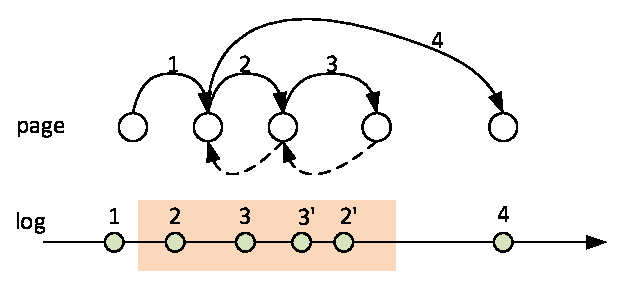
\includegraphics[width=0.6\linewidth]{handout/img/8-clr.eps}
    \caption{补偿日志}\label{fig:8-clr}
\end{figure}

CLR日志记录了对page对象的逆操作，它要指向前面的undo日志，以便应用该日志。同时undoNxtLSN指向CLR日志回退到的redo日志，这样系统重启后，可以直接跳过其间的日志条目，应用该CLR的下一条日志。如\figurename\ref{fig:8-clr}所示，$\{2, 3, 3', 2' \}$被跳过，$2'$下一条日志是$4$。

部分回滚牵涉到一个隐秘的问题，是否释放回滚部分获得的锁？如\figurename\ref{fig:8-clr}所示，$2, 3$获取行锁，$\{3', 2' \}$部分回滚后，这些锁需要释放。——这看起来违反了2PL协议，但是在道理上是讲得通的。如果不释放这些锁，由于扩大了事务资源的获取范围，死锁的风险会加大。

\subsection{swap}

如前所述，ARIES方案解耦了事务执行与缓冲管理，事务执行时，只需要关注对缓冲模块的操作，而缓冲模块的操作，只需要关注对磁盘的操作。在缓冲的设计中，一般不会允许缓冲容量无限制的增长，通常简单的做法是直接限制缓冲大小。

当缓冲不敷使用，就必须为新的页面请求腾挪出足够的空间。swap的策略很多，一般是直接使用lru，将lru队尾的页面换出，直到有足够的空间。lru并不管页面是否脏，干净页面直接释放，脏页面下刷。这些脏页面下刷，也需记录日志，可以将缓冲管理器看成一个内部事务，加入ATT表。

这些页面下刷的动作，仍然先写UNDO日志，REDO日志就不再需要了。注意到此时脏页面可能有未提交事务写入，所以数据库表并非只保存已提交事务的修改。数据库系统的状态并非只包含硬盘上的状态，而是硬盘+日志修正后的状态。

\begin{exercise}
    脏页面刷新，为什么不需要写REDO日志？
\end{exercise}

\figurename\ref{fig:8-swap}展示了脏页下刷，图中tid表示一个事务，buffer manager看成一个事务。所有日志条目看成日志流，这些日志条目抽象为堆。堆中的日志条目根据不同维度串联成链表，如按照事务，prevLSN串起了所有该事务的日志条目。另一个维度是页面，swap到磁盘上的页面，先UNDO一把，记录磁盘上之前的页面，当前LSN指向的日志包含一个指针指向上一个对该页面修改的日志。

\begin{figure}[H]
    \centering
    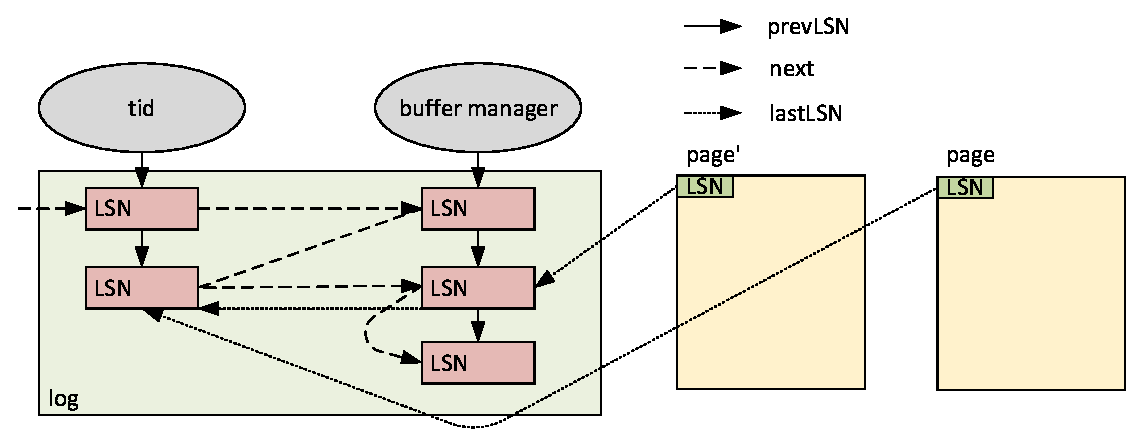
\includegraphics[width=\linewidth]{handout/img/8-swap.eps}
    \caption{脏页下刷}\label{fig:8-swap}
\end{figure}

日志格式是灵活的，在堆模型下，可以按照需要调整日志格式，如\figurename\ref{fig:8-swap}所示，日志中包含了对页面的修改，以及对页面的逆操作。

\section{Checkpoint}

检查点是需要的，日志文件长度不能无限增加，并且基于性能的考虑，系统自举后，要避免扫描日志开销过大。检查点是日志流中一类特殊的标记点，从它开始，系统可以重建。它是一个基线$b$，从它开始，每个日志条目代表一个对系统的修改$\Delta$，$b+\Delta_1+\Delta_2+...$最终重构系统状态。

\begin{figure}[H]
    \centering
    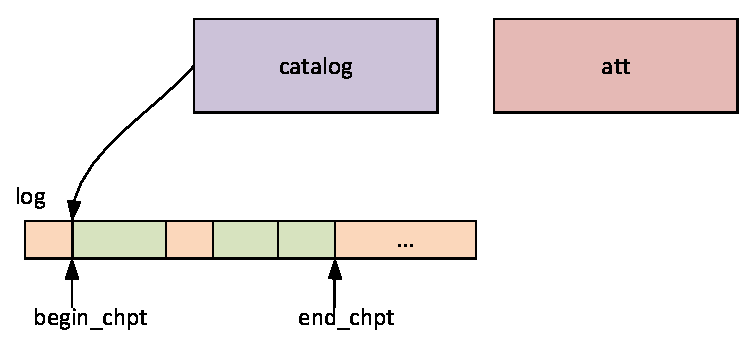
\includegraphics[width=0.6\linewidth]{handout/img/8-checkpoint.eps}
    \caption{fuzzy checkpoint}\label{fig:8-checkpoint}
\end{figure}

\subsection{fuzzy checkpoint}

早期的checkpoint构建要求系统松弛，即停止对外服务，找一个服务相对较少的时段，构建checkpoint，这称为sharp checkpoint。后来，发展出fuzzy checkpoint，以异步不停机方式构建checkpoint。

fuzzy checkpoint的实现方案如\figurename\ref{fig:8-checkpoint}所示，checkpoint被处理为一个内部事务。它启动后加入ATT表，构建过程中不断记录日志，构建完毕后，将catalog中的checkpoint位置指向begin\_ckpt的LSN。

checkpoint构建过程中，其它事务仍然执行，因此在日志流中，begin\_ckpt到end\_chpt之间可能会夹杂其它事务的日志。系统重启后，这些夹杂其间的日志会被识别出来，有些日志不会被redo，因为checkpoint在这些日志之后做总结。

接下去要考虑checkpoint需要做哪些基线。如\figurename\ref{fig:8-baseline}，首先是缓冲模块的脏页，这些页面要被写入磁盘，作为基线。其次是ATT表，它记录了系统当前活跃事务，这些事务要被写入磁盘。然后是catalog，对元数据的修改也需要记录在案，这些修改要被写入磁盘。

脏页面的处理除了交换到数据文件中，还需要转移一部分being\_chpt之前的UNDO日志到checkpoint上。脏页面的修改可能由ATT表上的活动事务做出，这些事务有被清退的可能，因此它们的修改UNDO日志要被转移到checkpoint上。

\begin{figure}[H]
    \centering
    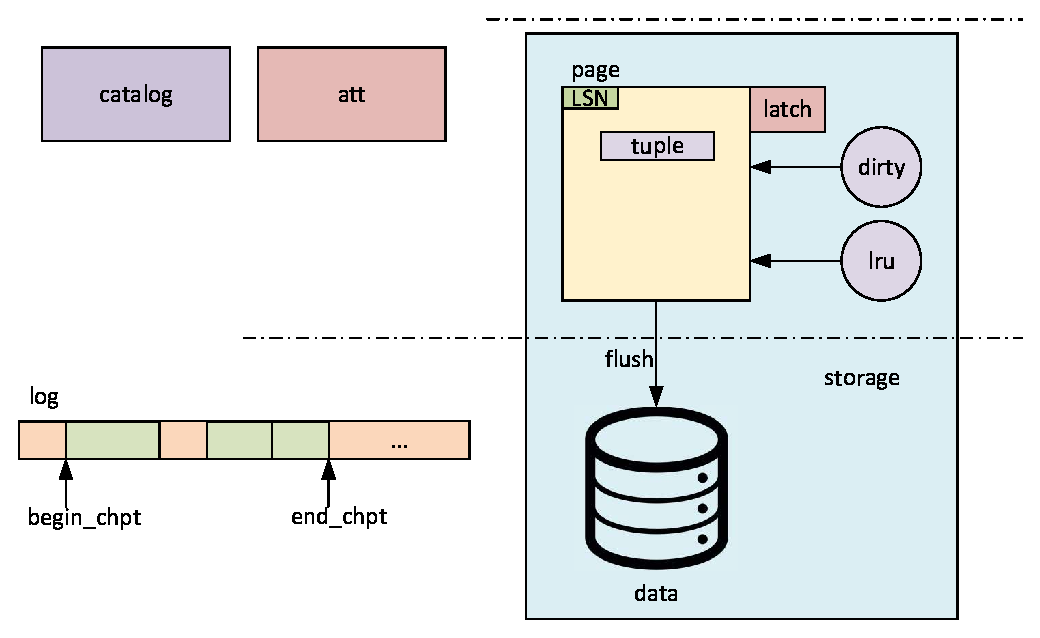
\includegraphics[width=0.8\linewidth]{handout/img/8-baseline.eps}
    \caption{checkpoint基线构建}\label{fig:8-baseline}
\end{figure}

打checkpoint需要将所有脏页落盘，这与缓冲管理层的flush功能不同，后者只是为了腾挪出足够的空间。checkpoint一般会周期性执行，也可以根据需要手动执行。

\begin{exercise}
    下刷了脏页，干净的页面怎么办？
\end{exercise}
\begin{exercise}
    checkpoint构建过程中，夹杂了部分其它事务修改记录，如何处理？如何识别哪些日志是需要在重启后redo？
\end{exercise}
\begin{exercise}
    前述的日志结构中，只有一个checkpoint类型，而checkpoint要执行的动作很多，这够吗？
\end{exercise}
\begin{exercise}
    打checkpoint，需要加锁吗？加latch的话，是否会影响其它事务的执行？
\end{exercise}

\section{系统重启}

系统重启过程，ARIES\cite{mohan1992aries}规范为三轮：

\begin{itemize}
    \item 第1轮，分析。要找到最近的checkpoint，以它为基线开始重放，一般会在catalog中记录。有些系统会打开日志，不断向前扫描，直到最近的checkpoint。在分析轮，要拉起事务模块和缓冲模块，准备好ATT表和空闲页面队列。
    \item 第2轮，重做。从checkpoint开始，顺序重放日志。新的事务开始，将它加到ATT表，然后执行它的REDO动作和补偿动作。写入页面操作，要buffer manager会先读取页面，读取完毕后，会检查该页面的LSN是否小于当前LSN。如果大于当前LSN，是因为这个页面被缓冲管理交换过，参考\figurename\ref{fig:8-swap}，按照链表找到小于当前页面的UNDO加载。当事务提交或者取消，从ATT表中驱逐这个事务。
    \item 第3轮，清扫。当所有日志重放完毕，ATT表内所剩的事务为未完成事务，处理为取消。应用这些事务的UNDO操作，将页面回退到前一个LSN，回滚前要记录补偿日志。
\end{itemize}

\begin{exercise}
    catalog非常重要，如何确保它的安全？
\end{exercise}

